\chapter{General relativity and Gravity}

In the previous chapter we learned how Newton's laws and the concepts of space and time themselves are to be rethinked of when we want to study nature at speeds close to the speed of light. Einstein Special Relativity has proven to be succesful in describing a huge variety of phenomena, from time dilations and length contractions to collision of particles and the propagation of electromagnetic waves in vacuum and through matter. The one thing that it fails in explaining, though, and that we will need to understand in order to study Modern Cosmology, is gravity. In this chapter we will first give an overview on how gravity is thought about classically (as Newton did), then explaining why this picture is in contradiction with Special Relativity, and finally how Einstein solved the problem with his formulation of General Relativity.

\section{Newton's gravity}
The main reason that led Isacc Newton in formulating his theory of gravity in the 16$^{\mathrm{th}}$ century, was that at the time there was a pretty solid empirical understanding of the motion of celestial bodies (planets); at the time the astronomer Johannes Kepler inferred from his observations three empirical rules that seemed to describe very well the orbital motion of the planets in the solar system
\begin{enumerate}
\item \textit{First rule}: the planets move in elliptical orbits around the sun; the sun coincides with one of the focal points of the orbit
\item \textit{Second rule}: the vector that connects the sun and the planet, $\mathbf{r}$, swipes equal areas in equal amounts of time
\item \textit{Third rule}: the square of the orbital period $T$ is proportional to the cube of the semimajor axis of the orbit $a$, namely $T^2=ka^3$ with $k$ a suitable proportionality constant
\end{enumerate}
\begin{figure}
\begin{center}
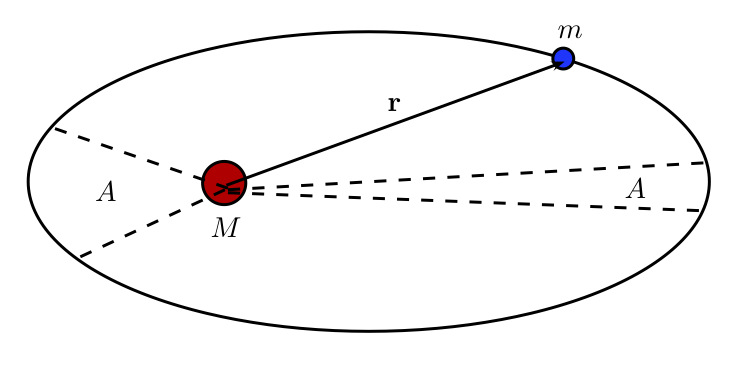
\includegraphics[scale=0.7]{Draw/kepler.png}
\label{}
\end{center}
\caption{Schematic representation of a planet's orbit: the gravitational force is always directed along the line that joins the planet and the sun; for this reason angular momentum is conserved and if the two arcs highligthened by dashed lines are covered in equal time intervals, than also the swiped areas, $A$, are the same}
\label{kepler}
\end{figure}
Newton formulated his theory of gravity with these three rules in mind as a guidance; what he came up with is that gravity is an attractive force between two bodies, it's always directed along the line that joins the objects and it's directly proportional to the product of their masses and inversely proportional to the square of their distance. With the reference of Figure \ref{kepler}, the planet, of mass $m$, according to Newton, feels an attractive force $\mathbf{F}_g$ from the sun, of mass $M$ given by
\begin{equation}
\label{newtgrav}
\mathbf{F}_g=-\frac{GmM}{r^2}\hat{\mathbf{r}}
\end{equation} 
Where the $G$ is a universal constant (Newton's constant) that was first measured by Cavendish in 1797 to be $G=6.67\times 10^{-11}\,\mathrm{m}^3\mathrm{kg}^{-1}\mathrm{s}^{-2}$; roughly speaking, Newton figured out that if rule 2 had to be satisfied then the orbital angular momentum of the planet had to be conserved during the orbit. This means that the gravitational force needs to be \textit{central} (i.e. directed along the line that connects the two bodies); the fact that orbits were closed ellipses with the force center in one of the focal points told him that only a $1/r^2$ dependence would do the trick (this is complicated to show, but you can take for granted that a $1/r^n$ dependence doesn't give closed orbits in general). Once established this, the third rule follows as a consequence of equation (\ref{newtgrav}): one can show that the proportionality constant $k$ depends only on the mass of the sun $k=\frac{4\pi^2}{GM}$. This theory of gravity explains basically all the solar system physics (except 
the orbit of mercury), from whose observations it was deduced; this has nevertheless some flaws. First of all, it violates special relativity; as if this wasn't enough, modern astronomical techiques pointed out the existence of several astrophysical systems for which a description in terms of newtonian gravity fails. We shall explore these concepts in the following paragraph. 

\section{The need for a new description}
In this paragraph we will try to understand the main flaws of Newton's gravity and why do we need a new description to understand the physics of the universe at its largest scales. As a first impression, you may notice that there is already a problem with equation (\ref{newtgrav}), in which the speed of light $c$ doesn't appear explicitely. Since in all relativity the speed of light plays a crucial role, the fact that this is not included in Newton's formulation already tells us that there will be some problems in conciliating the two pictures. Equation (\ref{newtgrav}) has however a worse problem: what it implies, in fact, is that gravity travels at infinite speed and any changes that occur on the sun are instantaneously reflected on all the surrounding planets (this is the so called \textit{action at a distance} problem). Since Einstein tells us (and there is also very solid experimental evidence) that no signal can travel faster than the speed of light, this is in explicit violation with relativity. For 
example, if our sun, which is 8 light minutes away from us, had to blow apart, earth wouldn't feel any effect until 8 minutes from the explosion at best. This feature is not captured by equation (\ref{newtgrav}). 
\subsection{The breakdown limit}
We can give some rough estimates on which is the limit above which Newtonian gravity is not reliable anymore; these estimates have to involve the speed of light, which is not included in the newtonian description. Consider a compact object (a planet, a star,...) of mass $M$ and radius $R$; using equations (\ref{centripetal}) and (\ref{newtgrav}) we can try to calculate the orbital speed $v$ for a circular orbit of radius $\gtrsim R$ using $\frac{v^2}{R}=\frac{GM}{R^2}$ which gives us $v=\sqrt{\frac{GM}{R}}$. This velocity scale is not very meaningful, what is meaningful though is the quantity $v_f=v\sqrt{2}$ which is the \textit{escape speed} from the object's surface: this is the minumum speed you need to give a rocket for it to escape the gravitational pull of the object. If the object were earth, for example, the escape speed from its surface would be $v_f=11.6$\,km/s; what if the object is much more compact and the escape velocity from it approaches $c$? This is precisely when newtonian gravity breaks 
down: a compact object so massive that $v_f=c$ is called a \textit{black hole} and it cannot be described in any way by newtonian gravity. $v_f=c$ is equivalent to say
\begin{equation}
\label{stronggrav}
\frac{GM}{Rc^2}=\frac{1}{2}
\end{equation} 
This will be our thumb rule for estimating when newton gravity breaks down: each time we have a system of mass $M$ and typical size $L$, we compute the ratio $\frac{GM}{Lc^2}$: if this ratio is much less than one ($v_f\ll c$) than we are fine, otherwise we need to come up with a better description of gravity. Let's give a few examples to have an idea on when this is the case
\begin{table}[htbp]
\begin{center}
\begin{tabular}{|c|c|c|c|} \hline
\textbf{System} & \textbf{Mass}($M$) & \textbf{Size}($L$) & \textbf{Ratio} $GM/Lc^2$ \\ \hline
The sun & $M_\odot\approx 2\cdot 10^{30}$\,kg & $7\cdot10^5$\,km &$10^{-5}$ \\ \hline
A typical neutron star & $M_\odot$ & 10\,km &1/3 \\ \hline
The universe (density $\rho \approx 10^{-30}\mathrm{g}\,\mathrm{cm}^{-3}$)& $\rho d_H^3$ & $d_H=H_0/c$ &$G\rho/H_0^2\approx 0.1\div0.5$ \\ \hline

\end{tabular}
\end{center}
\caption{A few estimates for newtonian gravity validity}
\end{table}
And we see that, even if for the sun Newton's gravity is perfectly acceptable as a description, when we move to more dense objects like neutron stars we really need to look for a better model. This is true also for the universe: if we want to study it at its largest observable scales and understand its key properties, newtonian gravity is not reliable. Before exploring the solution to this problem (which is Einstein general relativity), let's appreciate the fact that even if it works very well, newtonian gravity has some little flaws also in the solar system: for example, it fails in predicting some key features in Mercury's orbit. Mercury is the closest solar system planet to the sun and hence it's the one on which general relativistic effects are expected to be bigger; observationally Mercury's orbit exibits a very curious phenomenon, which is called \textit{perihelion precession}. Since for the gravitational force Mercury experiences from the sun is not exactly $\propto 1/r^2$, but it gets some non 
negligible general relativistic corrections $\propto 1/r^4$, its orbit is not exactly an ellipse, but it's an ellipse which perihelion (closest point of approach to the sun) is shifting (or preceding). This shift is very small ($43''$/century) but it's indeed observable and agrees with the prediction given by general relativity (that gives a number of order $GM_\odot/ac^2$ with $a$ the semimajor axis of the orbit).  

\section{A new picture for spacetime}
By the end of the previous paragraph you should have convinced yourselves that for understanding the universe at its largest observable scales, we need a new understanding of gravity and spacetime itself; we will do that going over the main ideas of General Relativity, who was developed by Einstein in 1920s and has proven to be very succesful in explaining the deviations from newtonian gravity. \footnote{For a quick sketchy introduction to the subject you can watch this very nice lecture from Brian Greene, who is one of the faculty here at Columbia \url{http://www.youtube.com/watch?v=0rocNtnD-yI}} What Einstein understood after careful thinking, is that gravity is nothing else but the manifestation of the geometry of spacetime itself; in the following, we will quantify this "geometry" concept in precise mathematical terms. For now, think about the following simple example illustrated in Figure \ref{freefall}.  
\begin{figure}
\begin{center}
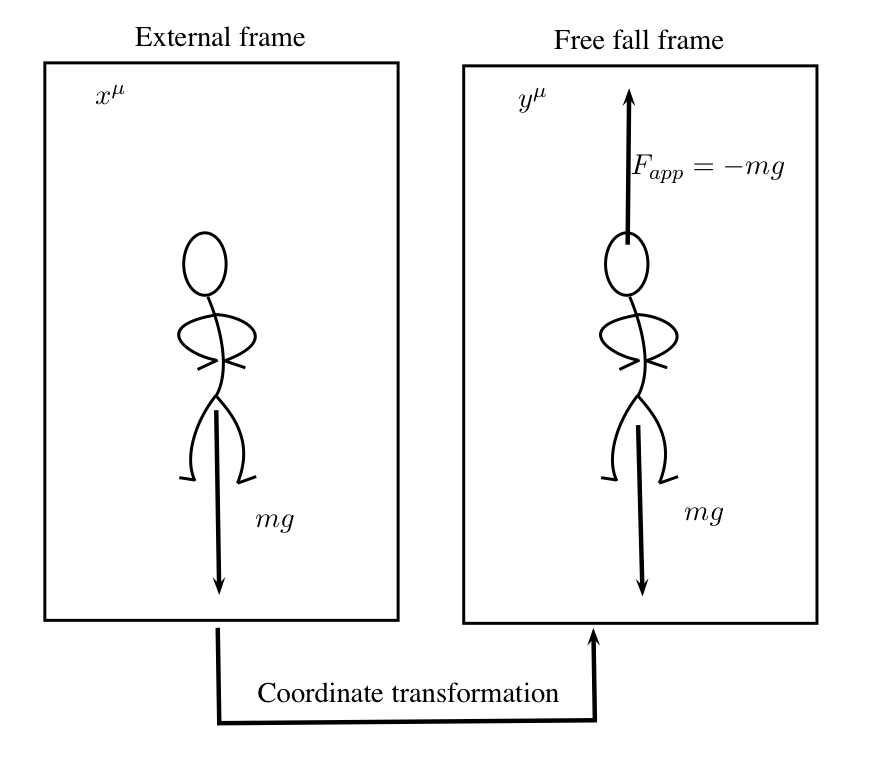
\includegraphics[scale=0.7]{Draw/Free_fall.png}
\label{}
\end{center}
\caption{A guy in a free falling elevator experiencing a zero total force}
\label{freefall}
\end{figure}
A guy is climbing a building in an elevator, at a certain time the elevator breaks and it starts to free fall under earth's gravity. As seen from an external observer, the guy (assuming he's not in contact with the floor) will experience the gravity force $mg$ and hence will accelerate towards the ground. From the accelerating elevator point of view, though, there will be an additional appearent force pointing up and exactly balancing gravity, due to the fact that we are looking at the situation from the point of view of a frame which itself accelerates with acceleration $g$. If we call $x^\mu$ the coordinates (space and time) in the external frame and $y^\mu$ the coordinates in the free falling frame, we see that the coordinate transformation $x\rightarrow y(x)$ brings us from a system in which gravity is present to a system in which gravity is absent. Paraphrasing this in mathematical terms, we can say that, in $y$ coordinates we can express the interval as
\begin{equation}
ds^2=\eta_{\mu\nu}dy^\mu dy^\nu
\end{equation}
We cannot the say the same in $x$ coordinates: we know that the interval $ds^2$ is invariant under coordinate transformations, but since $y$ and $x$ are not connected by a simple lorentz transformation (acceleration is involved), the best we can do is to write $ds^2=\eta_{\mu\nu}dy^\mu dy^\nu=g_{\mu\nu}dx^\mu dx^\nu$ where $g_{\mu\nu}$ is a symmetric $4\times4$ matrix, but it is not in the form \ref{etamunu}. What our coordinate transformation does for us, is that \textit{locally} (in the elevator), it transforms the complicated metric $g_{\mu\nu}$ into the flat one $\eta_{\mu\nu}$. General Relativity is based on this simple idea: this transformation always exists, i.e. it always exists a \textit{local free fall frame} (the analogous of the elevator idea can be applied for example to a spaceship falling in a black hole or on the space shuttle orbiting the earth; why is this a free fall frame?). This is the so called \textit{equivalence principle} which says that, given a generic point in spacetime $x$, in 
which the metric is $g_{\mu\nu}(x)$, it \textit{always} exists a coordinate transformation $y(x)$ such that, \textit{at the point} $y(x)$, the metric is transformed as $g'_{\mu\nu}(y(x))=\eta_{\mu\nu}$. To be a little bit more technical here, by \textit{metric transformation} we intend that, given the fact that the interval is invariant, $ds^2=g_{\mu\nu}(x)dx^\mu dx^\nu=g'_{\mu\nu}(y(x))dy^\mu dy^\nu$, the metric transforms in the way
\begin{equation}
g'_{\mu\nu}=g_{\alpha\beta}\frac{dx^\alpha}{dy^\mu}\frac{dx^\beta}{dy^\nu}
\end{equation}
The important statement here is that, in general, this transformation that locally cancels gravity does the trick $g_{\mu\nu}\rightarrow \eta_{\mu\nu}$ \textit{only at one point}; in general we can't find a coordinate transformation that cancels gravity at every point in space, and this makes sense, because if this would have been possible gravity wouldn't exist at all. For example, thinking back at the guy in the elevator, in his free fall frame he doesn't feel earth's gravity, but if he were to be sensible enough he could still feel the moon's gravitational pull (and the pull from the rest of the solar system as well). Now a tricky question arises: let's consider a generic metric $g_{\mu\nu}$ which describes our spacetime; it might be that $g_{\mu\nu}$ has a special form, such that I can revert it back to $\eta_{\mu\nu}$ all over the place using a particular coordinate transformation. Consider for example the following: 
\begin{equation}
\label{metspher}
ds^2=-c^2dt^2+dr^2+r^2(d\theta^2+\sin^2{\theta}d\phi^2)
\end{equation}
The metric here is not in the form $\eta_{\mu\nu}$, because it depends on the position $x^\mu=(ct,r,\theta,\phi)$; if we go from the spherical coordinates to the cartesian ones through the transformation (see Figure \ref{coordinates}) $(ct,r,\theta,\phi)\rightarrow(ct,x=r\sin{\theta}\cos{\phi},y=r\sin{\theta}\sin{\phi},z=r\cos{\theta})$, we can revert the metric back to the flat form 
\begin{equation}
ds^2=-c^2dt^2+dx^2+dy^2+dz^2
\end{equation}
\begin{figure}
\begin{center}
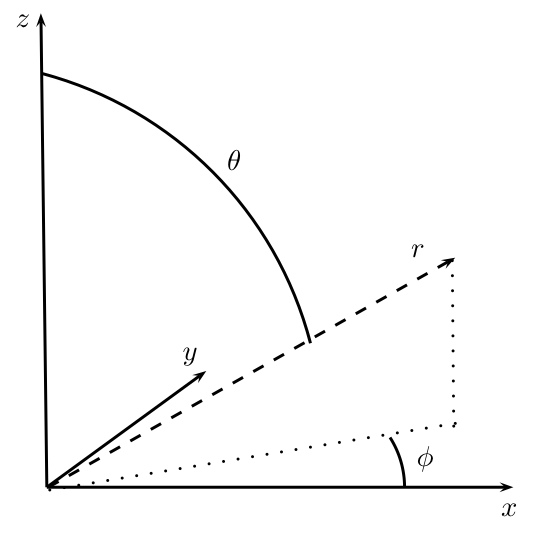
\includegraphics[scale=0.7]{Draw/coordinates.png}
\label{}
\end{center}
\caption{Spherical coordinate system}
\label{coordinates}
\end{figure}
This means that a metric in the form (\ref{metspher}), describes a spacetime which is flat, i.e., in which there are no gravitational forces, even if the metric depends on position. Consider now the following metric
\begin{equation}
\label{blackmetric}
ds^2=-c^2\left(1-\frac{2GM}{rc^2}\right)dt^2+\frac{dr^2}{1-\frac{2GM}{rc^2}}+r^2(d\theta^2+\sin^2{\theta}d\phi^2)
\end{equation}
It can be shown that there exists \textit{no coordinate transformation} that reverts this metric back to $\eta_{\mu\nu}$ in \textit{every} point in space; this is because this metric describes a spacetime in which there is a gravitational source (in particular a star or planet of mass $M$ in this case) and the spacetime is not flat. The question now is: given a generic metric $g_{\mu\nu}(x)$, how can we tell if it describes a flat spacetime or a spacetime is which there is gravity; once again Einstein helps us. The answer is that gravity manifests itself as \textit{curvature} in the spacetime bulk. As we wil understand later, a metric in the form (\ref{blackmetric}) is curved, whereas one in the form (\ref{metspher}) has no curvature and is flat. What do we precisely mean by this? And how do we know if a metric is curved? We will answer this question in the folowing paragraph. 
\subsection{The geometry of spacetime}
In the previous paragraph we have seen that choosing arbitrary coordinate reference frames (which are not necessarily connected by lorentz transformations), changes the metric $g_{\mu\nu}$ in such a way that the interval $ds^2$ is invariant; in this paragraph we want to convince ourselves that the metric $g_{\mu\nu}$ carries all the geometrical information on our spacetime. In particular the metric will do two things for us: 
\begin{itemize}
\item It will tell us how physical bodies should move (i.e. how planets orbit stars, black holes, etc.)
\item It will tell us when and how our spacetime is curved: this will tell us when we are, or we are not, in the presence of a gravitational source
\end{itemize}
Motivated by the study of special relativity, Einstein came up with these two rules for body motions in a spacetime with coordinate $x^{\mu}$ and metric $g_{\mu\nu}$; each physical body will follow a trajectory $x^{\mu}(s)$ such that 
\begin{enumerate}
\item If the body is massles (like a photon, i.e. a light ray) then the trajectory will satisfy $ds^2=g_{\mu\nu}dx^{\mu}dx^{\nu}\equiv 0$; this is the same as saying that massless particles travel at the speed of light
\item If the body has a mass then the trajectory will always satisfy $ds^2<0$ (the body will travel slower than light); moreover, among all the trajectories that connect two points $A$ and $B$, the body will choose that particular trajectory such as 
\begin{equation}
\Delta s_{AB}=\int_A^Bds
\end{equation}
is maximum. All such trajectories are called \textit{geodesics} and are determined entirely by the metric $g_{\mu\nu}$.
\end{enumerate}
The fact that bodies travel along geodesics can be paraphrased saying that bodies, when they move, "follow the geometry of spacetime"; since the metric shapes the trajectories, we can say that the metric encodes the geometry of spacetime. This gives us some insight on how gravity works in this new picture: the sun "curves" the spacetime, modifiying his metric. Planets must follow the geodesic dictated by the metric and hence orbit the sun. But how does the sun curve the spacetime around it? Before answering this question we must first understand what "curvature" actually means. 
\subsection{The meaning of curvature}
Let's think about the following example, involving simple geometrical ideas: a plane is flat, but a sphere is curved. What makes a sphere curved? And more important, can we distinguish a flat plane from a curved sphere just looking at their \textit{intrinsic} properties? (i.e. can we realize that a sphere is curved just sitting on it, without looking at it from the exterior?) It turns out we can, just look at Figure \ref{sphere}
\begin{figure}
\begin{center}
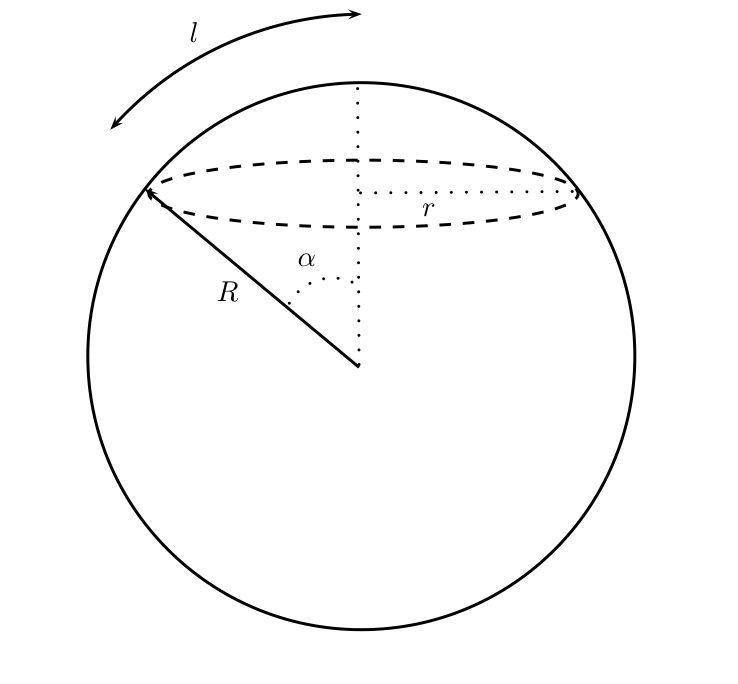
\includegraphics[scale=0.7]{Draw/sphere.png}
\end{center}
\caption{Example on why a sphere is curved}
\label{sphere}
\end{figure}
Suppose we have a rope of length $l$ which we fix, at one extreme, at the north pole; sitting on the sphere, we can measure two things: the length of the dashed circle (which is the collection of all the points touched by the rope as we go around one full turn) and the area on the sphere enclosed by it. Suppose that we know the value of $\pi$; let's call $C$ and $A$ the length of the circle and the area that we physically measure sitting on the sphere. If we were on a plane we would expect $C=2\pi l$ and $A=\pi l^2$, but looking again at Figure \ref{sphere}, you can convince yourselves that this is not the case. In fact we have (take the second relation for granted)
\begin{equation}
C=2\pi R\sin{\alpha}=2\pi R\sin{\left(\frac{l}{R}\right)}
\end{equation}
\begin{equation}
A=R^2\int_0^{2\pi}d\phi\int_0^{\alpha}\sin{\theta}d\theta=2\pi R^2(1-\cos{\alpha})=2\pi R^2\left[1-\cos{\left(\frac{l}{R}\right)}\right]
\end{equation}
And the relative corrections from the results we obtain on flat space are
\begin{equation}
\frac{C}{2\pi l}=\frac{R}{l}\sin{\left(\frac{l}{R}\right)}
\end{equation} 
\begin{equation}
\frac{A}{\pi l^2}=2\left(\frac{R}{l}\right)^2\left[1-\cos{\left(\frac{l}{R}\right)}\right]
\end{equation}
Now imagine that the radius $R$ of the sphere is very big, so big that if our rope is not so big, we barely notice the change: for $\alpha=l/R\ll 1$ we Taylor approximate $\sin{\alpha}\approx \alpha - \alpha^3/6$ and $\cos{\alpha}\approx1-\alpha^2/2+\alpha^4/24$ and we get 
\begin{equation}
\frac{C}{2\pi l}\approx 1-\frac{1}{6}\left(\frac{l}{R}\right)^2
\end{equation}
\begin{equation}
\frac{A}{\pi l^2}\approx 1-\frac{1}{12}\left(\frac{l}{R}\right)^2
\end{equation}
These relations tell us a couple of interesting facts:
\begin{itemize}
\item If the radius of the sphere is really big, and we don't go to far from the center with our rope, we barely notice the difference from being on a regular flat plane
\item The measurements of length and area that we get on the sphere are \textit{smaller} than those that we get on the plane (look at the minus sign): we conventionally refer this type of curvature as \textit{positive} curvature
\item Whatever curvature is, it's characterized by a length scale, in this case the radius of the sphere $R$, and all the corrections from flat space are proportional to $l^2$ that is to say to the area enclosed by our experiment
\end{itemize}
Believe it or not, these three facts will be enough to get a basic understanding on where the curvature comes in when we consider a spacetime metric $g_{\mu\nu}$ 
\begin{figure}
\begin{center}
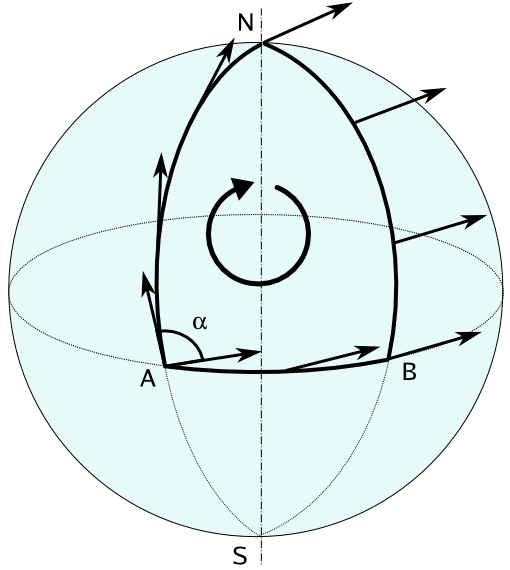
\includegraphics[scale=0.5]{Draw/Parallel_transport.png}
\end{center}
\caption{Parallel transport of a vector around a closed loop $A\rightarrow B\rightarrow N \rightarrow A$: on a curved space the vector will be tilted when it comes back to $A$, and the tilt will be proportional to the area enclosed by the loop. Source \url{http://en.wikipedia.org/wiki/File:Parallel_transport.png}}
\label{transport}
\end{figure}
Consider a situation similar to Figure \ref{transport}; you can generalize this conclusions to an arbitrary curved space: consider a vector $v^\mu$, and a closed loop $ABNA$ on the surface. Imagine to \textit{transport} this vector around the loop in such a way that, on each part of the loop, the vector forms a constant angle with the \textit{tangent} to the loop; this way of moving vectors is called \textit{parallel transport}. When the vector comes back to the original point, if the surface is curved, it will be tilted, and this tilt will be proportional to the area enclosed by the loop. Now consider a very small loop of sides $dx^\mu$ and $dx^\nu$ like in Figure \ref{loop}
\begin{figure}
\begin{center}
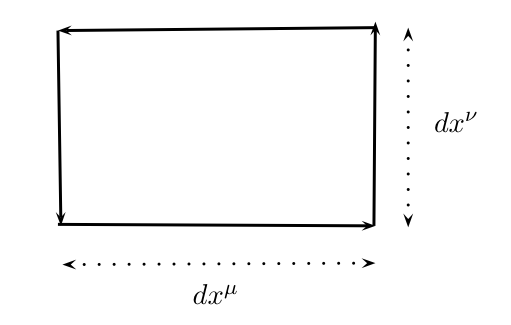
\includegraphics[scale=0.8]{Draw/loop.png}
\end{center}
\caption{A small loop on a curved surface}
\label{loop}
\end{figure}
If we parallel transport a vector along this loop it will undergo a change $\Delta v^\lambda$ proportional to the area $dx^\mu dx^\nu$; the change will also be proportional to the vector itself, since if we transport a vector with all zero components, it make sense that the transported vector will remain zero. Hence the change must be proportional to $\Delta v^\lambda\propto v^\rho dx^\mu dx^\nu$; the thing that we miss is the curvature, i.e. the 1/(length scale)$^2$; since we want this to be an invariant statement, we see that the curvature cannot be a simple number, but must be at least a tensor with 4 indices, and this must have measure units (length)$^{-2}$, this will be the first rigorous definition of curvature we encounter
\begin{equation}
\Delta^{loop}v^\lambda=R_{\mu\nu\rho}^\lambda v^\rho dx^\mu dx^\nu
\end{equation}
This $R_{\mu\nu\rho}^\lambda$ is called \textit{riemann tensor} and we claim that it can be calculated \textit{directly} from the metric: it measures the curvature, in the sense that if it is 0 then the space is flat and there are no gravitational sources, but if it is non zero then it means that the space is curved and there must be some curving source in it. The fact that the riemann tensor can be calculated directly from the metric is due to the fact that, given a geodesic, it can be shown that its tangent vector is parallel transported along it. Since geodesics are defined by the metric and are connected to parallel transport, then the curvature must be expressed as some (even if complicated) function of the metric. Once we understand this, then the jump to the final new picture of gravity is simple (but it took Einstein to make it!): the sun (and matter in general) curves the space around the planets. The planets' orbits are the geodesics in this curved metric. The statement "matter curves space" is 
expressed mathematically as Einstein equation, which has the general form
\begin{equation}
\label{einsteinsymb}
\mathrm{(Some \,\,function\,\, of }\,R_{\mu\nu\lambda}^\rho[g_{\mu\nu}] \mathrm{ \,\,and\,\, } g_{\mu\nu})= \mathrm{(Some\,\, tensor \,\,that\,\, describes\,\, matter)}
\end{equation}
Describing the motion of planets now becomes the following process: find the sun's distortion to the flat metric solving Einstein's equation (\ref{einsteinsymb}) and then find the geodesics in this metric. In the solar system this method gives results which are very close to the newtonian ones, except that contrary to Newton, the Einstein's equation predicts the correct Mercury's perihelion precession.